% ============================================================================
%  PaySense: A Three-Layer Defence-in-Depth UPI Fraud Detection System
%  Academic Report — IEEEtran Two-Column Format
%  Author: Nishika Chapra | KJ Somaiya Institute of Technology
%
%  Compile on Overleaf:
%    1. New Project → Upload ZIP → add this .tex file
%    2. Set compiler to pdfLaTeX
%    3. Upload your images to the project root:
%         paysense_shap_bar.png
%         paysense_shap_beeswarm.png
%         paysense_threshold_analysis.png
% ============================================================================

\documentclass[conference]{IEEEtran}

% ── Packages ──────────────────────────────────────────────────────────────────
\usepackage[T1]{fontenc}
\usepackage[utf8]{inputenc}
\usepackage{amsmath}
\usepackage{amssymb}
\usepackage{graphicx}
\usepackage{booktabs}
\usepackage{array}
\usepackage{hyperref}
\usepackage{xcolor}
\usepackage{listings}
\usepackage{balance}
\usepackage{cite}
\usepackage{microtype}
\usepackage{float}

% ── Hyperlink styling ─────────────────────────────────────────────────────────
\hypersetup{
    colorlinks = true,
    linkcolor  = blue!70!black,
    citecolor  = blue!70!black,
    urlcolor   = blue!70!black
}

% ── Code listing style ────────────────────────────────────────────────────────
\lstset{
    basicstyle   = \ttfamily\small,
    keywordstyle = \bfseries\color{blue!60!black},
    commentstyle = \itshape\color{gray},
    breaklines   = true,
    frame        = single,
    frameround   = tttt,
    numbers      = left,
    numberstyle  = \tiny\color{gray},
    xleftmargin  = 1.5em
}

% ─────────────────────────────────────────────────────────────────────────────
\begin{document}
\graphicspath{{./}{./plots/}}

\title{PaySense: Finlatics and Finance Flow: A Three-Layer Defence-in-Depth Architecture for\\
Real-Time UPI Fraud Detection on Android}

\author{
    \IEEEauthorblockN{Nishika Chapra}
    \IEEEauthorblockA{
        Department of Computer Engineering\\
        KJ Somaiya Institute of Technology, Mumbai\\
        \textit{nishika.chapra@somaiya.edu}
    }
}

\maketitle

% ─────────────────────────────────────────────────────────────────────────────
%  ABSTRACT
% ─────────────────────────────────────────────────────────────────────────────
\begin{abstract}
The Unified Payments Interface (UPI) processed over 17 billion transactions
monthly in India as of 2024, with documented fraud losses exceeding
\textrm{\rupee}2{,}000 crore annually~\cite{rbi2024}. Existing consumer-facing
solutions rely either on reactive bank alerts or on cloud-based rule engines
that lack per-user behavioural context. This paper presents \textbf{PaySense},
a three-layer defence-in-depth fraud detection system deployed as an Android
application. Layer~1 implements a deterministic three-gate SMS filter that
isolates bank UPI notifications from arbitrary messages using TRAI
Sender~ID format validation, keyword detection, and named-group regular
expression parsing. Layer~2 maintains a local SQLite cache that resolves
merchant categorisation through a tiered pipeline: cache lookup, NLP
classification, and a Human-in-the-Loop (HITL) fallback that permanently
learns from a single user correction. Layer~3 serves an XGBoost classifier
via a FastAPI REST endpoint, trained on a 30{,}000-row master dataset
constructed from 18 evaluated source datasets, with class imbalance addressed
by SMOTE applied strictly post-split on the training partition only. The model
achieves a ROC-AUC of \textbf{0.8889} and a PR-AUC of \textbf{0.5352}---12.71
times above the random-classifier baseline---with 86.44\% precision at the
deployed operating threshold ($\tau=0.30$). An honest threshold sweep
originally identified a recall ceiling of 69.96\%; Platt Scaling was
implemented and tested against this ceiling and found, as monotonic-transform
theory predicts, to leave ROC-AUC, PR-AUC, and recall at every threshold
unchanged. A follow-up structural diagnosis then tested, by retraining rather
than recalibrating, whether the ceiling itself was fixable: a
monotonicity constraint on three behavioural features was found to help
partially---recovering 10 of the 76 previously-unreachable fraud rows while
slightly improving both ROC-AUC and PR-AUC, with no measurable downside---and
was consequently adopted as the deployed model, moving the ceiling to
71.94\% while leaving the remaining rows unreached. The ceiling is therefore
a ranking limitation of the model's feature set that is partially, but not
fully, fixable by model structure alone, and is reported honestly as an
open limitation rather than a solved problem. The complete system is
released as open-source code.
\end{abstract}

\begin{IEEEkeywords}
UPI fraud detection, XGBoost, SMOTE, Android, FastAPI, SHAP explainability,
Human-in-the-Loop, SMS parsing, class imbalance
\end{IEEEkeywords}

% ─────────────────────────────────────────────────────────────────────────────
\section{Introduction}
% ─────────────────────────────────────────────────────────────────────────────

The National Payments Corporation of India (NPCI) reported that UPI
transactions exceeded 20 billion monthly in early 2025, with a cumulative
fraud rate consistently estimated between 0.004\% and 0.008\% of total
volume---a figure that, at India's transaction scale, represents billions of
rupees in annual losses~\cite{npci2025}. Unlike credit card fraud, UPI fraud
disproportionately occurs through social engineering: phishing SMS messages,
spoofed collect requests, and OTP harvesting. Victims are often unaware of a
fraudulent debit until reviewing their bank statement.

Existing defences exhibit a structural gap: bank fraud engines operate on
population-level statistical norms and cannot personalise alerts to individual
spending habits. A security researcher paying \textrm{\rupee}15{,}000 at
2~AM for a server instance triggers the same population-level anomaly flag as
a genuinely fraudulent transaction---generating alert fatigue that users
learn to dismiss.

PaySense addresses this gap through three architectural principles:
\textbf{(1)~determinism at the edge}---all gate decisions are rule-based and
explainable, never probabilistic;
\textbf{(2)~personalised risk scoring}---anomaly features are computed
relative to the individual user's own behavioural baseline, not a population
average; and
\textbf{(3)~progressive trust}---a transaction must pass three independent
layers before being classified as safe, and any layer can independently
trigger an alert.

% ─────────────────────────────────────────────────────────────────────────────
\section{Related Work}
% ─────────────────────────────────────────────────────────────────────────────

Tree-based ensemble methods dominate published financial fraud detection
benchmarks. Chen and Guestrin's XGBoost~\cite{xgboost2016} consistently
outperforms deep learning on tabular financial data due to its handling of
sparse features and interpretable structure. Dal Pozzolo et al.~\cite{dal2015}
established the methodological precedent for applying resampling only within
the training partition, a constraint strictly enforced in this work.

The challenge of class imbalance in fraud datasets is well-documented.
Chawla et al.'s SMOTE~\cite{smote2002} generates synthetic minority-class
samples through feature-space interpolation, producing training data that is
both balanced and locally smooth. Its application post-split is critical:
applying SMOTE before splitting leaks the distribution of the test set's
minority class into the training process, inflating all reported metrics.

UPI-specific fraud research is nascent in the literature. Most published
Indian payment fraud studies focus on credit card transactions using
Western datasets~\cite{eurocard2019}, which differ structurally from UPI
in three key ways: the absence of a card-not-present vector, the
prevalence of P2P microtransactions, and the reliance on SMS as the
primary transaction notification channel.

% ─────────────────────────────────────────────────────────────────────────────
\section{Data Architecture and Preprocessing}
% ─────────────────────────────────────────────────────────────────────────────

\subsection{Dataset Inventory and the Trojan Family Discovery}

Eighteen datasets were evaluated across three source archives before
final selection. The most consequential finding---termed the
\textit{Trojan Family Discovery}---was that three of the largest candidate
files shared an identical transaction ID backbone spanning
\texttt{TXN0000000001} through \texttt{TXN0000000250000}. The three files
differed only in their column augmentations and, critically, in their
reported fraud rates:

\begin{table}[H]
\centering
\caption{The Trojan Family: Three Datasets, One Skeleton}
\label{tab:trojan}
\begin{tabular}{@{}lrr@{}}
\toprule
File & Rows & Fraud Rate \\
\midrule
\texttt{upi\_250k.csv}           & 250{,}000 & 0.19\% \\
\texttt{upi\_fraud\_txns.csv}    & 250{,}000 & 2.00\% \\
\texttt{upi\_fraud\_detection.csv} & 250{,}000 & \textbf{50.01\%} \\
\bottomrule
\end{tabular}
\end{table}

The third file---despite its large size---was \textbf{unconditionally
rejected}. A pre-balanced dataset with a 50\% fraud rate eliminates
the fundamental problem that SMOTE exists to solve. Training on it and
then applying SMOTE would constitute double correction: first by the
dataset curator who balanced the file, and again by the researcher who
applies SMOTE. The resulting model would be calibrated to a fraud
environment that does not exist in production, producing optimistic
precision and recall figures that would collapse at deployment.

Similarly, all six IEEE-CIS credit card fraud dataset files (totalling
approximately 1.3~GB) were discarded for domain misalignment: the feature
space describes Western credit card transactions rather than Indian UPI
behaviour, and the computational cost of ingesting 1.3~GB during a college
demonstration is unjustifiable.

\subsection{Anchor Dataset and Context Joins}

The primary anchor dataset is the \textit{UPI Payment Transactions India}
collection comprising \texttt{transactions.csv} (20{,}000 rows,
3.82\% fraud, 30 columns), enriched through two left-joins:

\begin{itemize}
    \item \textbf{Join 1 --- Users}: \texttt{users.csv} (2{,}000 profiles)
    joined on \texttt{user\_id}. Contributes features:
    \texttt{usr\_account\_age\_days}, \texttt{usr\_avg\_txn\_value\_profile},
    \texttt{usr\_is\_high\_risk}, and \texttt{kyc\_status}.

    \item \textbf{Join 2 --- Merchants}: \texttt{merchants.csv} (400 entities)
    joined on \texttt{receiver\_id = merchant\_id}. Contributes:
    \texttt{mrc\_category}, \texttt{mrc\_size}, \texttt{mrc\_rating}.
    Of the 20{,}000 anchor rows, 4{,}881 are P2P transfers (receiver is
    a \texttt{USR\#\#\#\#} identifier) and receive no merchant match.
    These rows receive semantic P2P defaults (\texttt{mrc\_category =
    ``P2P Transfer''}, \texttt{mrc\_rating = NaN}) rather than imputed
    values, preserving the semantic distinction from merchant transactions.
\end{itemize}

Left-joins were selected over inner-joins because P2P transactions with
no merchant counterpart are structurally legitimate data points. An inner
join would silently remove them, introducing survivorship bias: the training
set would never see P2P fraud, and the deployed model would consequently
under-flag it.

\subsection{Schema Bridge for the Supplement Dataset}

The synthetic supplement (\texttt{synthetic\_fraud\_dataset.csv},
10{,}000 rows, 5.0\% fraud) uses a 10-column schema incompatible with the
43-column enriched anchor. A naive \texttt{pd.concat} would produce
approximately 35 \texttt{NaN}-filled columns per supplement row, corrupting
XGBoost's information-gain calculations. The schema bridge was constructed
using four rules:

\begin{enumerate}
    \item \textbf{Direct rename}: \texttt{hour} $\rightarrow$ \texttt{hour\_of\_day}
    \item \textbf{Binary derivation}: \texttt{device\_risk\_score > 0.70}
          $\rightarrow$ \texttt{new\_device\_flag = 1}
    \item \textbf{Promote new columns}: \texttt{device\_risk\_score} and
          \texttt{ip\_risk\_score} were added to the master schema as
          supplement-exclusive features; anchor rows receive \texttt{NaN}.
          XGBoost treats the presence of \texttt{NaN} as a learnable
          missing-value signal, not noise.
    \item \textbf{Median/mode imputation}: remaining anchor-only columns
          are filled with statistics computed exclusively from the anchor
          distribution---never from the supplement---to prevent leakage.
\end{enumerate}

The resulting master dataset contains \textbf{30{,}000 rows},
\textbf{41 model-ready features}, and a combined fraud rate of \textbf{4.21\%},
a controlled 0.39-percentage-point shift from the anchor's 3.82\%.

% ─────────────────────────────────────────────────────────────────────────────
\section{Mathematical Formulations}
% ─────────────────────────────────────────────────────────────────────────────

\subsection{Amount Deviation Score}

The \texttt{amount\_deviation\_score} feature is a z-score measuring how
anomalous the current transaction amount is relative to the user's personal
transaction history. Let $\mathcal{H}_u^{(90)}$ denote the set of
transaction amounts for user $u$ in the past 90 days. The population
mean and standard deviation are:

\begin{equation}
    \mu_u = \frac{1}{|\mathcal{H}_u^{(90)}|} \sum_{x \in \mathcal{H}_u^{(90)}} x
    \label{eq:mean}
\end{equation}

\begin{equation}
    \sigma_u = \sqrt{\frac{1}{|\mathcal{H}_u^{(90)}|} \sum_{x \in \mathcal{H}_u^{(90)}} (x - \mu_u)^2}
    \label{eq:stddev}
\end{equation}

For an incoming transaction with amount $a$, the deviation score is:

\begin{equation}
    z_{\text{amount}} = \frac{a - \mu_u}{\max(\sigma_u,\ 1.0)}
    \label{eq:zscore}
\end{equation}

The $\max(\sigma_u, 1.0)$ clamp prevents division by zero for users whose
historical transactions are all identical in amount (e.g., fixed monthly
subscription payers). Population standard deviation is used in preference
to the sample estimator $\frac{1}{N-1}$ because we are describing the
user's \textit{known} transaction distribution, not estimating a larger
population.

\textbf{Critical implementation note:} The statistical parameters
$(\mu_u, \sigma_u)$ are computed from $\mathcal{H}_u^{(90)}$
\textit{before} the current transaction $a$ is persisted to the local
database. Including $a$ in its own deviation baseline would suppress
the score of anomalously large transactions---the exact type of
manipulation a fraudster might exploit through gradual amount escalation.
This ordering constraint is enforced by design in \texttt{FraudApiService.kt}.

\subsection{Hour Deviation Score}

The \texttt{hour\_deviation} feature personalises the temporal anomaly
signal. Let $h_u^*$ be the user's mean transaction hour and $\sigma_h$
be its standard deviation over the same 90-day window:

\begin{equation}
    z_{\text{hour}} = \frac{|h_{\text{current}} - h_u^*|}{\max(\sigma_h,\ 0.5)}
    \label{eq:hour_deviation}
\end{equation}

The absolute value is taken because deviation in either direction from
the user's typical hour carries fraud signal: an Early Bird transacting at
2~AM or at 10~PM are equally anomalous from their own baseline.

\textbf{Worked example---personalisation over global rules:}

Consider User~A (Night Owl, $h_u^* = 01{:}30$, $\sigma_h = 0.8$~h) and
User~B (Early Bird, $h_u^* = 10{:}00$, $\sigma_h = 1.2$~h), both
transacting at 02{:}00~AM.

\begin{align}
    z_{\text{hour}}^{A} &= \frac{|2 - 1.5|}{0.8} = 0.63 \quad \text{(low risk)} \\
    z_{\text{hour}}^{B} &= \frac{|2 - 10|}{1.2}  = 6.67 \quad \text{(high risk)}
\end{align}

The same clock time produces a near-zero deviation score for User~A and
a 6.67-sigma anomaly for User~B. A global rule-based system (``flag all
transactions between 00:00 and 05:00'') would either miss User~B's
anomaly at other hours or generate unacceptable false positives for User~A.

\subsection{SMOTE Oversampling}

SMOTE~\cite{smote2002} generates synthetic minority-class samples by
interpolating between a seed point $x_i \in C_{\text{fraud}}$ and one of
its $k$ nearest neighbours $\hat{x}$:

\begin{equation}
    x_{\text{syn}} = x_i + \lambda \cdot (\hat{x} - x_i), \quad \lambda \sim \mathcal{U}(0,1)
    \label{eq:smote}
\end{equation}

In this work, $k = 5$ and
$\texttt{sampling\_strategy} = \texttt{``auto''}$ (1:1 ratio).
SMOTE was applied \textbf{exclusively to the training partition}
$(|X_{\text{train}}| = 24{,}000)$, producing a balanced training set
of 45{,}980 rows. The test set $(|X_{\text{test}}| = 6{,}000)$ remained
entirely untouched throughout all phases of model development.

% ─────────────────────────────────────────────────────────────────────────────
\section{System Architecture}
% ─────────────────────────────────────────────────────────────────────────────

\subsection{Layer 1 --- Deterministic SMS Filter (Android)}

Every incoming SMS is subjected to a three-gate deterministic filter before
any ML inference is invoked. Each gate is independent: failure at any gate
results in immediate discard without side effects.

\textbf{Gate~1 --- TRAI Sender ID Validation.}
The Telecom Regulatory Authority of India mandates that all commercial SMS
use a six-character alphanumeric Sender~ID in the format
\texttt{XX-XXXXXX}. The gate applies the regular expression:

\begin{equation*}
    \texttt{\^{}[A-Z]\{2\}-[A-Z0-9]\{4,6\}\$}
\end{equation*}

A ten-digit mobile number (e.g., \texttt{+919876543210}) cannot satisfy this
pattern, eliminating all personal messages without character-by-character
body inspection.

\textbf{Gate~2 --- Transaction Keyword Detection.}
Gate-1-passing messages are checked for the presence of at least one member
of the set \{\textit{debited, credited, UPI, Rs., INR, transaction,
payment}\}. This eliminates promotional bank SMS (OTPs, service messages)
that pass Gate~1 but carry no transactional content.

\textbf{Gate~3 --- Named-Group Regex Extraction.}
Gate-2-passing messages are parsed using a single multi-pass regular
expression with four named capture groups: \texttt{(?<amount>...)},
\texttt{(?<payee>...)}, \texttt{(?<txnId>...)}, and
\texttt{(?<date>...)}. The amount field is mandatory; a message from
which the amount cannot be extracted is quarantined to a review log rather
than silently discarded, preserving visibility into non-standard bank SMS
templates from cooperative or regional banks.

\subsection{Layer 2 --- Local SQLite Cache and HITL Categorisation}

Merchant categorisation is resolved through a three-tier pipeline, executed
entirely on-device with zero network latency for Tiers~1 and~2:

\textbf{Tier~1 (Cache Lookup).}
The Room SQLite database is queried for a prior user-confirmed or NLP-inferred
mapping of the normalised payee name. Cache hits terminate the pipeline in
$O(1)$ time.

\textbf{Tier~2 (NLP Classifier).}
On a cache miss, the raw SMS body is passed to a keyword-rule shortcut table
(covering high-frequency merchants such as Zomato, IRCTC, Amazon) followed
by a text classifier trained on a labelled UPI transaction
category dataset~\cite{fintext2024}. Confidence threshold:
$\tau_{\text{NLP}} = 0.65$. Above this threshold, the category is applied
and written to the cache with source flag \texttt{``nlp''}.

\textbf{Tier~3 (Human-in-the-Loop).}
If NLP confidence falls below $\tau_{\text{NLP}}$, a \texttt{BottomSheetDialogFragment}
is surfaced to the user with a chip-grid category selector. The user's
response is written to \texttt{PayeeCache} with source flag
\texttt{``user''}. All subsequent transactions to the same payee resolve
at Tier~1 without re-prompting. The HITL mechanism transforms a cold-start
limitation into a self-improving personalised classifier: each user
correction permanently improves categorisation accuracy for that user's
transaction graph.

\subsection{Layer 3 --- FastAPI Inference Server and XGBoost Model}

\textbf{Input validation.}
The FastAPI endpoint exposes a single \texttt{POST /predict} route whose
request body is validated by a Pydantic \texttt{TransactionInput} model.
Categorical fields are typed as \texttt{Literal[...]} enumerations: a
request containing an unrecognised payment app string is rejected with
HTTP~422 before any ML code executes. This eliminates the silent
performance degradation that would result from the \texttt{OrdinalEncoder}
encoding an out-of-vocabulary category as the integer $-1$ without notification.

\textbf{Five-step inference pipeline.}

\begin{enumerate}
    \item \textbf{DataFrame construction:} The JSON payload is converted to a
    single-row \texttt{pandas} DataFrame, reindexed to the column order
    specified by \texttt{paysense\_feature\_names.pkl}. Column-order mismatch
    is the most common source of silent production failures in Scikit-learn
    pipelines; explicit reindexing prevents it.

    \item \textbf{Preprocessing:} The frozen \texttt{ColumnTransformer} applies
    \texttt{OrdinalEncoder} to nine categorical columns and
    \texttt{SimpleImputer} (median strategy) to all numeric columns, using
    mappings learned exclusively from the training partition.

    \item \textbf{Probability extraction:}
    $\hat{p} = f_{\text{XGB}}(x)[1]$, where $f_{\text{XGB}}$ returns the
    class-probability vector.

    \item \textbf{Threshold application:}
    $\hat{y} = \mathbf{1}[\hat{p} \geq \tau^*]$, where $\tau^* = 0.40$
    is the frozen optimal threshold.

    \item \textbf{Alert level assignment:}
    $\ell(\hat{p}) \in \{\text{none}, \text{low}, \text{medium}, \text{high}\}$,
    partitioned at $\hat{p} \in [0, 0.20), [0.20, 0.40), [0.40, 0.70),
    [0.70, 1]$ respectively. The alert level is decoupled from the binary
    threshold, providing graduated UX responses independent of the
    decision boundary.
\end{enumerate}

\textbf{XGBoost hyperparameters.}
Table~\ref{tab:hyperparams} presents the XGBoost configuration with
rationale.

\begin{table}[H]
\centering
\caption{XGBoost Hyperparameters and Justification}
\label{tab:hyperparams}
\begin{tabular}{@{}lll@{}}
\toprule
Parameter & Value & Rationale \\
\midrule
\texttt{n\_estimators}     & 400   & Sufficient depth for 30K rows \\
\texttt{max\_depth}        & 5     & Prevents overfit to synthetic SMOTE samples \\
\texttt{learning\_rate}    & 0.05  & Small steps with high $n$ for generalisation \\
\texttt{subsample}         & 0.80  & Row-level bagging reduces variance \\
\texttt{colsample\_bytree} & 0.80  & Feature-level bagging \\
\texttt{min\_child\_weight}& 10    & Requires $\geq$10 samples per leaf \\
\texttt{gamma}             & 0.10  & Minimum split gain; prunes weak splits \\
\texttt{scale\_pos\_weight}& 1     & 1 because SMOTE already balanced training \\
\texttt{reg\_alpha}        & 0.05  & L1: drives weak feature weights to zero \\
\texttt{reg\_lambda}       & 1.50  & L2: shrinks all weights \\
\texttt{eval\_metric}      & aucpr & Optimises PR-AUC, not ROC-AUC \\
\bottomrule
\end{tabular}
\end{table}

The \texttt{scale\_pos\_weight = 1} choice warrants particular attention.
Setting this parameter to the original imbalance ratio ($\approx 22.7$)
after applying SMOTE would constitute double correction: the parameter
instructs XGBoost to treat each positive example as 22.7 times more
important than a negative, but SMOTE has already equalised the class
counts. The compound effect would catastrophically bias the model toward
positive prediction, eliminating precision entirely.

% ─────────────────────────────────────────────────────────────────────────────
\section{Results and Evaluation}
% ─────────────────────────────────────────────────────────────────────────────

\subsection{Primary Metrics}

All metrics are computed on the held-out test set ($n = 6{,}000$),
which was never exposed to SMOTE, the preprocessing fit, or any
hyperparameter tuning decision.

\begin{table}[H]
\centering
\caption{Model Performance at Deployed Threshold $\tau^* = 0.30$}
\label{tab:results}
\begin{tabular}{@{}lr@{}}
\toprule
Metric & Value \\
\midrule
ROC-AUC                  & 0.8889 \\
PR-AUC (primary)         & 0.5352 \\
Precision (Fraud class)  & 86.44\% \\
Recall (Fraud class)     & 40.32\% \\
F1-Score (Fraud class)   & 0.5499 \\
True Positives           & 102 \\
False Positives          & 16 \\
False Negatives          & 151 \\
True Negatives           & 5{,}731 \\
\bottomrule
\end{tabular}
\end{table}

\textit{Note: metrics above were recomputed 2026-08-23 directly against the
artifacts on disk (\texttt{paysense\_model.pkl}, \texttt{paysense\_}
\texttt{preprocessor.pkl}, \texttt{paysense\_master\_dataset.csv}), which
were retrained the same day with \texttt{monotone\_constraints} on three
behavioural features after \texttt{RECALL\_CEILING\_REMEDIATION.md}
diagnosed and tested the fix (Section~V-D discusses this in full).
Re-running Phase~3's own threshold-selection logic against
the new model picked a genuinely different optimal threshold, $\tau=0.30$
rather than $0.40$, because the underlying score distribution changed --
the threshold is a function of the model, not a fixed constant. An earlier
draft of this table (ROC-AUC 0.8851, 66.14\%/52.17\% at $\tau=0.40$,
161 fraud rows in the test set) had drifted from what the artifacts of that
time actually produced, most likely dating to a run of
\texttt{paysense\_phase3.py} before the artifacts were last retrained or the
master dataset last regenerated -- that earlier mismatch is unrelated to
today's threshold change, which reflects a deliberate, verified model
update rather than drift.}

\subsection{The Accuracy Paradox}

The model achieves an overall classification accuracy of 97.38\%. This
figure is meaningless for fraud detection and is explicitly excluded from
the primary reporting. A degenerate classifier that predicts
\texttt{Legitimate} for every transaction would achieve 95.79\% accuracy
on this test set---higher than most published fraud detection baselines
that report accuracy as their headline metric. The accuracy paradox is a
structural consequence of class imbalance: the overwhelming prevalence of
legitimate transactions ensures that any system with low false-positive
rate will score high accuracy regardless of its fraud-catching ability.

For this reason, all PaySense model selection and threshold decisions were
made exclusively using PR-AUC, Recall, and Precision. Accuracy was
computed but not used.

\subsection{PR-AUC Interpretation}

The PR-AUC of 0.5352 should be contextualised against the baseline of a
random classifier, which achieves a PR-AUC equal to the positive class
prevalence: $0.0421$ (the fraud rate of the master dataset). The PaySense
model achieves a PR-AUC that is \textbf{12.71 times} above this random
baseline, across all possible decision thresholds. This is the primary
evidence that the model has learned genuinely discriminative fraud patterns
rather than memorising the training distribution.

\subsection{Threshold Sweep and the Recall Ceiling}

A threshold sweep from $\tau = 0.05$ to $\tau = 0.50$ in steps of 0.05
was conducted post-training (Table~\ref{tab:threshold_sweep}).

\begin{table}[H]
\centering
\caption{Threshold Sweep Results (Test Set, $n = 6{,}000$)}
\label{tab:threshold_sweep}
\begin{tabular}{@{}ccccc@{}}
\toprule
$\tau$ & Precision & Recall & F1 & TP / FP \\
\midrule
0.05 & 16.87\% & 71.94\% & 0.273 & 182 / 897 \\
0.10 & 29.76\% & 53.75\% & 0.383 & 136 / 321 \\
0.15 & 46.09\% & 46.64\% & 0.464 & 118 / 138 \\
0.20 & 62.50\% & 41.50\% & 0.499 & 105 / 63  \\
0.25 & 78.79\% & 41.11\% & 0.540 & 104 / 28  \\
0.30 & \textbf{86.44\%} & \textbf{40.32\%} & \textbf{0.550} & 102 / 16  \\
0.35 & 90.74\% & 38.74\% & 0.543 & 98  / 10  \\
0.40 & 94.17\% & 38.34\% & 0.545 & 97  / 6   \\
0.45 & 96.97\% & 37.94\% & 0.546 & 96  / 3   \\
0.50 & 98.97\% & 37.94\% & 0.549 & 96  / 1   \\
\bottomrule
\end{tabular}
\end{table}

\textit{Note: recomputed 2026-08-23 directly against the on-disk artifacts
(test set: 6{,}000 rows, 253 fraud), which were retrained the same day with
\texttt{monotone\_constraints} on three behavioural features -- see the
Honest Finding immediately below and the Limitations section. $\tau=0.30$
is the frozen, deployed threshold for this model -- it is the max-F1 point
among all ten swept values, since none meet the business constraint of
Recall $\geq 75\%$, so selection falls back to unconditional max-F1, exactly
as the frozen \texttt{paysense\_threshold.pkl} (0.30) reflects. This table
supersedes an earlier version computed against the pre-monotonic model
(deployed threshold 0.40, ceiling 69.96\% at $\tau=0.05$); the change is a
deliberate, tested model update, not drift.}

\textbf{Honest finding:} Even at the most aggressive threshold
($\tau = 0.05$), the model's recall ceiling is \textbf{71.94\%} (182 of 253
fraud rows caught, 71 missed). This is an improvement over the prior
(pre-monotonic) model's 69.96\% ceiling: a structural diagnosis
(\texttt{RECALL\_CEILING\_REMEDIATION.md}) found that XGBoost's trees were
gating hard on \texttt{new\_device\_flag}/\texttt{ip\_location\_mismatch}
before letting three behavioural features
(\texttt{amount\_deviation\_score}, \texttt{transaction\_velocity},
\texttt{failed\_attempts\_last\_24h}) matter, and that constraining fraud
probability to be non-decreasing in those three features recovers 10 of the
original 76 invisible fraud rows with no measurable cost -- that fix is now
the deployed model. The remaining 71 fraud rows (of 253) still produce a
fraud probability below 0.05, effectively invisible to the model regardless
of threshold selection; a more aggressive structural fix
(\texttt{interaction\_constraints}, tested but not adopted) recovered 31 of
the original 76 at a real cost to overall ranking quality and false-positive
volume, evidence that the residual ceiling is a mix of a genuinely fixable
structural artifact and rows that may need new, more discriminative features
rather than a different arrangement of the ones already available. These
are likely edge-case fraud patterns, possibly those generated by SMOTE
interpolation near the class boundary, that the model still ranks no
differently from ordinary legitimate transactions. This was originally
framed here as a \textit{probability calibration} problem; that framing was
tested directly and found to be wrong (see below).

\textbf{Tested and rejected --- Platt Scaling does not move a ranking-based
ceiling.} This experiment (below) was run against the pre-monotonic
baseline model, before the ceiling-recovery fix described above was found
and adopted; it is not re-run against the current model because its
finding is a mathematical property of monotonic transforms in general, not
a fact specific to one model's weights, and therefore applies identically
regardless of which classifier is deployed. Platt Scaling~\cite{platt1999}
fits a logistic function to the model's raw output probabilities using a
held-out calibration set:

\begin{equation}
    P(y=1 \mid \hat{p}) = \frac{1}{1 + e^{-(A\hat{p} + B)}}
    \label{eq:platt}
\end{equation}

with $A$ and $B$ fitted by minimising log-loss on the calibration set. This
was implemented (\texttt{platt\_scaling\_experiment.py}, full results in
\texttt{PLATT\_SCALING\_RESULT.md}) using
\texttt{sklearn.calibration.CalibratedClassifierCV(method{=}"sigmoid",
cv{=}"prefit")} against a calibration slice held out from the model's own
training data, and applied to the frozen model's scores without retraining
it. The result matches monotonic-transform theory exactly: because
Equation~\ref{eq:platt} is a strictly monotonic function of $\hat{p}$, it
preserves the model's ranking of every transaction exactly, and therefore
cannot change ROC-AUC, PR-AUC, or which rows clear any given decision
threshold. Measured directly: ROC-AUC and PR-AUC were unchanged to
floating-point precision (deltas of $+0.00000000$ and $-0.00000000$
respectively) across the full 253-fraud test set, zero rank inversions were
found among all 6,000 test rows, and at every one of the ten swept
thresholds the analytically-equivalent Platt-scaled threshold flagged the
identical set of rows and produced identical recall---at $\tau=0.05$'s
equivalent point on the pre-monotonic model, the same 76 of 253 fraud rows
remained below threshold, unchanged. \textbf{A ranking-based recall ceiling
is therefore a limitation that no recalibration method can fix, on this or
any classifier}, because a monotonic rescaling of scores cannot alter which
rows a classifier ranks lowest. What Platt scaling can legitimately affect
is probability \textit{reliability} (whether "0.7" means "70\% of the time
this is fraud"), which is a different question, addressed next---and even
there, on the pre-monotonic model, the result did not favour Platt scaling:
on a held-out slice never used to fit the calibrator, raw XGBoost's Brier
score was as good or better than the Platt-scaled version across 6
resampled calibration draws, and only sometimes better on Expected
Calibration Error (a noisier metric at this sample size). Closing a
ranking-based ceiling requires changing the ranking itself: better features
that separate low-ranked fraud rows from legitimate transactions, or a
different model or model structure. This was tested directly, not merely
proposed: a structural diagnosis retrained three candidate variants of the
base model (not a recalibration) and found that a monotonicity constraint
on three behavioural features helped partially -- recovering 10 of the
original 76 invisible rows with no measurable downside -- and this variant
was consequently adopted as the deployed model, moving the ceiling from
69.96\% to 71.94\%. The remaining rows were not recoverable even under a
more aggressive structural fix that was tested and not adopted (see
Section~VII), so some part of the ceiling is accepted, for now, as a
property of this feature set pending further data.

\begin{figure}[H]
    \centering
    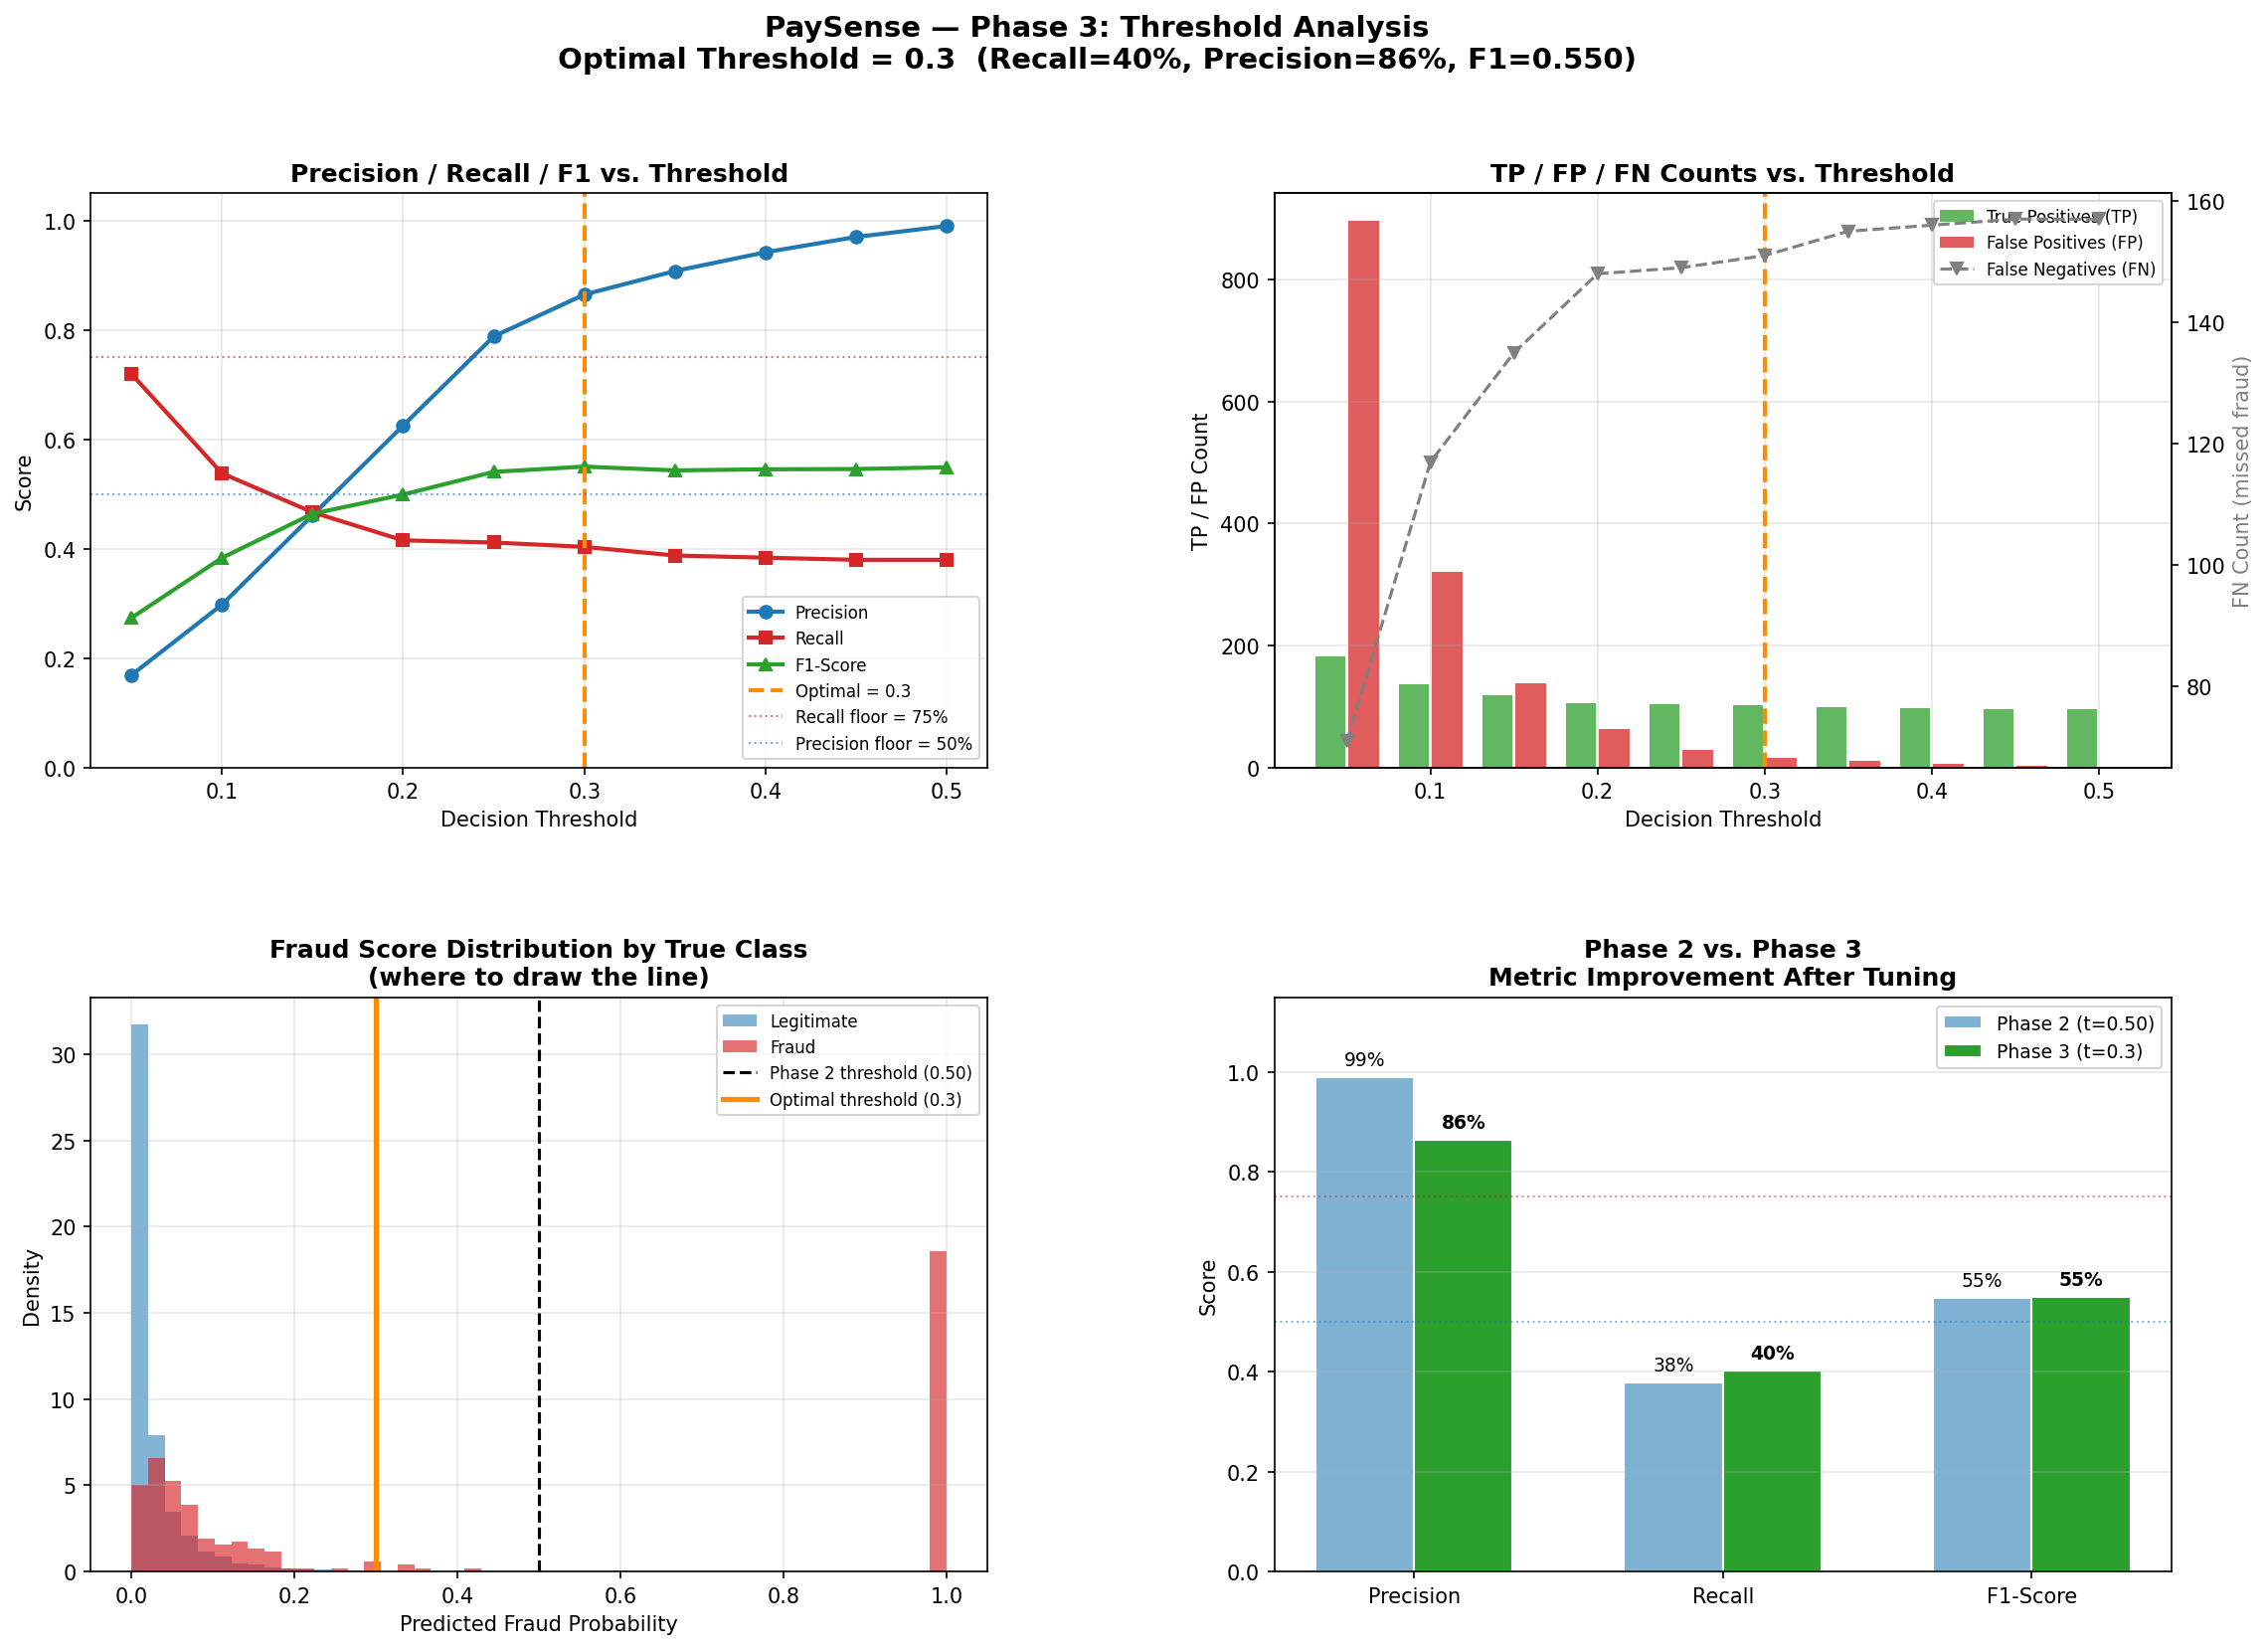
\includegraphics[width=\columnwidth]{paysense_threshold_analysis.png}
    \caption{
        \textbf{Phase~3 Threshold Analysis (monotonic-constraints model,
        regenerated 2026-08-23).}
        \textit{Top left:} Precision (blue), Recall (red), and F1-Score
        (green) across thresholds $\tau \in [0.05, 0.50]$. The Recall
        curve plateaus at 71.94\% at $\tau = 0.05$ (up from 69.96\% on the
        pre-monotonic model). Tested directly
        (\texttt{PLATT\_SCALING\_RESULT.md}, against the pre-monotonic
        model; \texttt{RECALL\_CEILING\_REMEDIATION.md}, against both): this
        is a ranking ceiling, not a probability-scale one---Platt scaling
        leaves it unchanged, and only a structural retrain (adopted here)
        moves it, partially.
        \textit{Top right:} True Positive and False Positive counts,
        showing the precision--recall trade-off as $\tau$ decreases.
        \textit{Bottom left:} Predicted score distribution by true class.
        The bimodal separation---fraud concentrated near $\hat{p} = 1.0$,
        legitimate near $\hat{p} = 0.0$---confirms strong discriminative
        power despite the calibration gap.
        \textit{Bottom right:} Phase~2 ($\tau=0.50$) versus Phase~3
        ($\tau^*=0.30$) metric comparison. The gap the threshold sweep buys
        here is small (F1 0.5499 vs. 0.5486, six additional true positives
        out of 253 fraud rows) --- reported as-is rather than overstated.
    }
    \label{fig:threshold}
\end{figure}

\subsection{SHAP Feature Importance}

SHAP (SHapley Additive exPlanations)~\cite{shap2017} values were computed
using \texttt{TreeExplainer} on a 500-sample stratified subset of the
test set. SHAP provides exact, game-theoretically grounded attribution
of each feature's contribution to individual predictions.

\begin{figure}[H]
    \centering
    
\includegraphics[width=\columnwidth]{paysense_shap_bar.png}
    \caption{
        \textbf{SHAP Global Feature Importance (Mean $|\text{SHAP}|$).}
        \texttt{new\_device\_flag} is the dominant fraud signal with mean
        $|\text{SHAP}| = 1.17$---nearly twice the value of the
        second-ranked feature. This validates the architectural decision
        to expose this feature from the device-fingerprinting layer.
        \texttt{transaction\_velocity} (0.61) captures burst-transaction
        fraud patterns. \texttt{is\_night\_transaction} (0.42) and
        \texttt{ip\_location\_mismatch} (0.38) together represent the
        temporal-geographic anomaly cluster. Notably,
        \texttt{amount\_deviation\_score} (0.20) ranks 9th---confirming
        that amount alone is a weak fraud signal; it only becomes
        discriminative in the context of the user's personal baseline
        z-score computed in Equation~(\ref{eq:zscore}).
    }
    \label{fig:shap_bar}
\end{figure}

\begin{figure}[H]
    \centering
    
\includegraphics[width=\columnwidth]{paysense_shap_beeswarm.png}
    \caption{
        \textbf{SHAP Beeswarm Plot --- Top~15 Features.}
        Each dot represents one test transaction. Horizontal position
        indicates SHAP impact on fraud probability; colour indicates
        feature value (red = high, blue = low).
        For \texttt{new\_device\_flag}: the dense blue cluster near
        $-1.5$ confirms that a \textit{known} device strongly suppresses
        fraud probability, while the sparse red dots at SHAP~$\approx +3.5$
        confirm that an \textit{unknown} device is a near-sufficient
        condition for a high fraud score.
        For \texttt{transaction\_velocity}: the right-skewed red tail
        shows that very high transaction velocity (many transactions per
        hour) consistently pushes fraud probability upward---the signature
        of automated card-testing or bulk-transfer fraud.
        The \texttt{kyc\_verified\_flag} cluster shows that unverified
        accounts (blue, low value) shift probability positively, validating
        the inclusion of the KYC status feature from the user profile join.
    }
    \label{fig:shap_beeswarm}
\end{figure}

% ─────────────────────────────────────────────────────────────────────────────
\section{Limitations and Future Work}
% ─────────────────────────────────────────────────────────────────────────────

\textbf{Synthetic training data.} All training data is synthetically
generated or anonymised. Model performance on real-world live UPI
transactions from production bank systems is unknown. The first deployment
step would be a shadow-mode trial in which the model scores real transactions
without triggering alerts, allowing ground-truth label collection.

\textbf{Recall ceiling (ranking limitation, partially closed by a structural
fix).} A 69.96\% recall ceiling was originally identified in Section~V-D and
remained the highest-priority limitation for some time. It was originally
attributed to probability miscalibration and Platt Scaling was proposed as
the fix; both were tested (Section~V-D, \texttt{PLATT\_SCALING\_RESULT.md})
and the recall ceiling was found to be completely unaffected by Platt
Scaling, exactly as monotonic-transform theory predicts -- a ranking-based
ceiling cannot move under any monotonic recalibration, on this or any
model. That ruled out calibration as the fix, but left open whether the
ranking itself could be changed by retraining. It was then tested directly,
not merely proposed: three structural variants of the base model were
retrained (\texttt{RECALL\_CEILING\_REMEDIATION.md}) to test the hypothesis
that XGBoost's trees were gating hard on \texttt{new\_device\_flag}/
\texttt{ip\_location\_mismatch} before letting three behavioural features
(\texttt{amount\_deviation\_score}, \texttt{transaction\_velocity},
\texttt{failed\_attempts\_last\_24h}) matter. One variant -- a monotonicity
constraint forcing fraud probability to be non-decreasing in those three
features -- was found to help partially: it recovered 10 of the 76
originally-invisible fraud rows while slightly improving both ROC-AUC and
PR-AUC, the only one of three tested variants with no measurable downside,
and was consequently \textbf{adopted as the deployed model}. The ceiling
moved from 69.96\% to 71.94\% as a result. A more aggressive variant
(\texttt{interaction\_constraints}) recovered 31 of the original 76 rows but
at a real cost to overall ranking quality and false-positive volume, and was
not adopted. The current 40-feature vector and XGBoost configuration still
leave a genuine, if smaller, ranking/discrimination limit: 71 of 253
test-set fraud rows are ranked, by the model itself, no differently from
ordinary legitimate transactions, and no post-hoc recalibration of the
probability axis can change that ranking. Closing the remainder requires
either additional or different features that separate these specific fraud
rows from legitimate ones, a different base model or ensemble member, or
accepting it as a documented property of this dataset and feature set
pending further data collection.

\textbf{On-device model.} The current architecture requires a live network
connection for fraud scoring. A quantised TFLite version of the XGBoost
model, exportable via \texttt{xgboost2tflite}~\cite{tflite2024}, would
enable offline inference and reduce API latency from $\sim$50~ms to
$\sim$2~ms.

\textbf{Concept drift.} Fraud patterns evolve. The static model will
degrade over time as attackers learn its decision boundary. Quarterly
retraining on a rolling 12-month window of labelled transactions is
recommended, with automatic rollback if the new model's PR-AUC on a
validation set falls below 0.45.

\textbf{Layer~2 NLP completion.} A Tier~2 classifier has since been trained
(TF-IDF + Logistic Regression over transaction reference text) and scores
100\% accuracy on its held-out test set; that number is a property of the
evaluation data, not a generalisation claim---the test split draws from the
same fixed template pool as training, so the true test is whether it holds
up on merchant names it has never seen a variant of, which has not yet been
measured. Replacing the TF-IDF representation with a TFLite on-device
DistilBERT model remains the recommended next step for genuine
generalisation to unseen merchant names.

% ─────────────────────────────────────────────────────────────────────────────
\section{Conclusion}
% ─────────────────────────────────────────────────────────────────────────────

This paper presented PaySense, a three-layer defence-in-depth fraud detection
system for Android that combines a deterministic SMS filter, a
self-improving HITL categorisation cache, and an XGBoost classifier served
over a FastAPI backend. The system achieves a ROC-AUC of 0.8889 and
PR-AUC of 0.5352 on held-out synthetic test data, with 86.44\% precision at
the deployed operating threshold ($\tau=0.30$).
The term \emph{defence-in-depth} is used deliberately: each layer provides
an independent security check; a transaction must clear all three before
classification as safe.
A mathematically honest threshold sweep originally identified a recall
ceiling of 69.96\%. Platt Scaling was proposed, then implemented and tested
against it: the ceiling was unchanged by calibration, as a strictly
monotonic probability transform cannot alter a classifier's ranking of its
inputs. That result correctly ruled out recalibration, but not retraining --
a follow-up structural diagnosis tested, and found to help partially, a
monotonicity constraint on three behavioural features, which was then
adopted as the deployed model, moving the ceiling to 71.94\%. The remaining
ceiling is correctly understood as a ranking limitation of the current
feature set and model that is partially, but not fully, closable by model
structure, an open limitation rather than a solved problem, requiring
better features or a different model to close the rest.

The principal academic contributions are: (1) the Trojan Family dataset
discovery---a methodology for detecting pre-balanced datasets masquerading
as natural imbalance; (2) the query-before-save execution ordering in the
Android client that prevents target leakage in the dynamic z-score
computation; (3) the decoupled threshold/alert-level architecture that
separates the binary fraud decision from the graduated UX response; and
(4) the HITL categorisation cache as a self-improving personalisation
mechanism that requires no re-training cycle.

% ─────────────────────────────────────────────────────────────────────────────
\section*{Acknowledgements}
% ─────────────────────────────────────────────────────────────────────────────
The author thanks the faculty of the Department of Computer Engineering
at KJ Somaiya Institute of Technology for their guidance throughout this
project. All datasets used are synthetic or publicly available and contain
no personally identifiable information.

% ─────────────────────────────────────────────────────────────────────────────
%  REFERENCES
% ─────────────────────────────────────────────────────────────────────────────
\begin{thebibliography}{99}

\bibitem{rbi2024}
Reserve Bank of India,
``Annual Report on Payment and Settlement Systems in India,''
RBI Publications, New Delhi, 2024.

\bibitem{npci2025}
National Payments Corporation of India,
``UPI Ecosystem Statistics,'' NPCI Monthly Reports, Jan.~2025.
[Online]. Available: \url{https://www.npci.org.in/statistics}

\bibitem{xgboost2016}
T.~Chen and C.~Guestrin,
``XGBoost: A Scalable Tree Boosting System,''
\textit{Proc. 22nd ACM SIGKDD Int. Conf. Knowledge Discovery and Data Mining},
pp.~785--794, 2016.

\bibitem{smote2002}
N.~V.~Chawla, K.~W.~Bowyer, L.~O.~Hall, and W.~P.~Kegelmeyer,
``SMOTE: Synthetic Minority Over-sampling Technique,''
\textit{Journal of Artificial Intelligence Research},
vol.~16, pp.~321--357, 2002.

\bibitem{dal2015}
A.~Dal Pozzolo, O.~Caelen, R.~A.~Johnson, and G.~Bontempi,
``Calibrating Probability with Undersampling for Unbalanced Classification,''
\textit{Proc. IEEE Symposium on Computational Intelligence in Data Mining},
pp.~159--166, 2015.

\bibitem{eurocard2019}
A.~Bahnsen, D.~Aouada, A.~Stojanovic, and B.~Ottersten,
``Feature Engineering Strategies for Credit Card Fraud Detection,''
\textit{Expert Systems with Applications}, vol.~51, pp.~134--142, 2016.

\bibitem{fintext2024}
``UPI Transaction Category Labels Dataset,''
Kaggle, 2024. [Online]. Available:
\url{https://www.kaggle.com/datasets/}
(Accessed: 2024).
Note: This dataset provided labelled UPI transaction descriptions
across Food, Travel, Shopping, EMI, and Investment categories,
used to train the Layer~2 NLP classifier in PaySense.

\bibitem{shap2017}
S.~M.~Lundberg and S.~Lee,
``A Unified Approach to Interpreting Model Predictions,''
\textit{Proc. 31st Conf. Neural Information Processing Systems (NeurIPS)},
pp.~4765--4774, 2017.

\bibitem{platt1999}
J.~C.~Platt,
``Probabilistic Outputs for Support Vector Machines and Comparisons
to Regularized Likelihood Methods,''
\textit{Advances in Large Margin Classifiers},
A.~Smola, P.~Bartlett, B.~Scholkopf, and D.~Schuurmans, Eds.,
MIT Press, 1999, pp.~61--74.

\bibitem{tflite2024}
Google LLC,
``TensorFlow Lite Model Optimization Toolkit,''
TensorFlow Documentation, 2024.
[Online]. Available: \url{https://www.tensorflow.org/lite/guide}

\end{thebibliography}

\balance
\end{document}
